\documentclass[10pt,a4paper]{article}
\usepackage[utf8]{inputenc}

% Define the page margin
\usepackage[margin=3cm]{geometry}

% Better typography (font rendering)
\usepackage{microtype}

% Math environments and macros
\usepackage{amsmath}
\usepackage{amsfonts}
\usepackage{amssymb}
\usepackage{amsthm}

% Define \includegraphics to include graphics
\usepackage{graphicx}

% Draw graphics from a text description
\usepackage{tikz}

% Syntax highlighting
\usepackage{minted}

% Set global minted options
\setminted{linenos, autogobble, frame=lines, framesep=2mm}

% Import the comment environment for orgtbl-mode
\usepackage{comment}

% Do not indent paragraphs
\usepackage{parskip}

\title{Distributed Systems, Sheet 6}
\author{Marten Lienen (03670270)}

\begin{document}

\maketitle

\section*{Exercise 1}

\subsection*{Part a)}

\begin{minted}{java}
  private int acks = 0;

  public synchronized void update(int clientId, Object value) {
    this.acks = 0;
    this.value = value;

    if (isPrimary) {
      for (Replica r : replicas) {
        r.update(clientId, value);
      }
    } else {
      sendAck(replicaId, clientId);
    }
  }

  public synchronized void receiveAck(int replicaId, int clientId) {
    acks++;

    if (acks == replicas.length()) {
      client.receiveAck();
    }
  }
\end{minted}

\subsection*{Part b)}

\subsubsection*{Scenario 1}

The value was successfully replicated and the client notified, so no steps have to be taken immediately.
Though if the client sends another request, it will notice that the previous primary is down and have to connect to a new primary.

\subsubsection*{Scenario 2}

The client will possibly retry the request after a timeout.
To that end it will first have to find the replacement primary, which will then have to recognize the query as a duplicate and send the acknowledgement right away.

\subsubsection*{Scenario 3}

Here again the client will probably retry the request at a new primary.
This new primary will then handle the request normally.

\subsubsection*{Scenario 4}

The scenario assumes that all backups have received the update, so the new primary has handled the original request and proceeds such as in scenario 2.

\section*{Exercise 2}

\begin{minted}{scala}
  // Client
  List replicas;

  def sendUpdate(value) {
    Message.sendTOBroadcast(value, replicas);
  }

  def receiveAck(msgId, replicaId) {
    // If the broadcast is reliable, it is enough to wait for one acknowledgement
    // for a given msgId because that means that all replicas have received the
    // update. Otherwise you would have to implement some resending of messages
    // with timeouts here.
  }

  // Message
  def sendTOBroadcast(message, recipients) {
    // Implement TO broadcasts with a global coordinator that assigns sequence numbers
  }

  def sendMessage(message, recipients) {
    // Send a message directly
  }

  // Replica
  def receiveUpdate(msgId, clientId, value) {
    storeValue(value);
    sendAck(clientId, msgId);
  }

  def sendAck(clientId, msgId) {
    Message.sendMessage(msgId, client.fromId(clientId));
  }
\end{minted}

\section*{Exercise 3}

\subsection*{Part a)}

I assume that an update message contains all updates and their update timestamps instead of just the latest value.
This way the recipient of a gossip message can apply the updates one after another.

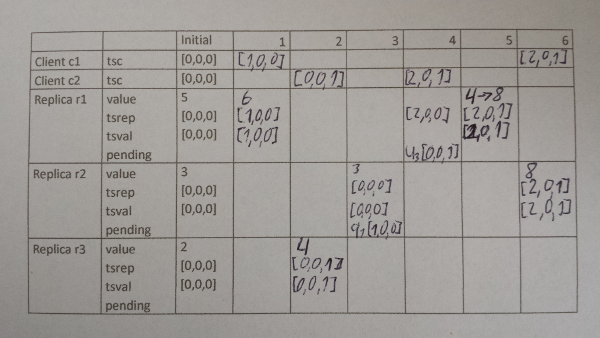
\includegraphics[width=\textwidth]{sheet-6/exercise-3-a}

\end{document}
